% Options for packages loaded elsewhere
\PassOptionsToPackage{unicode}{hyperref}
\PassOptionsToPackage{hyphens}{url}
\PassOptionsToPackage{dvipsnames,svgnames,x11names}{xcolor}
%
\documentclass[
]{article}
\usepackage{amsmath,amssymb}
\usepackage{lmodern}
\usepackage{iftex}
\ifPDFTeX
  \usepackage[T1]{fontenc}
  \usepackage[utf8]{inputenc}
  \usepackage{textcomp} % provide euro and other symbols
\else % if luatex or xetex
  \usepackage{unicode-math}
  \defaultfontfeatures{Scale=MatchLowercase}
  \defaultfontfeatures[\rmfamily]{Ligatures=TeX,Scale=1}
\fi
% Use upquote if available, for straight quotes in verbatim environments
\IfFileExists{upquote.sty}{\usepackage{upquote}}{}
\IfFileExists{microtype.sty}{% use microtype if available
  \usepackage[]{microtype}
  \UseMicrotypeSet[protrusion]{basicmath} % disable protrusion for tt fonts
}{}
\makeatletter
\@ifundefined{KOMAClassName}{% if non-KOMA class
  \IfFileExists{parskip.sty}{%
    \usepackage{parskip}
  }{% else
    \setlength{\parindent}{0pt}
    \setlength{\parskip}{6pt plus 2pt minus 1pt}}
}{% if KOMA class
  \KOMAoptions{parskip=half}}
\makeatother
\usepackage{xcolor}
\IfFileExists{xurl.sty}{\usepackage{xurl}}{} % add URL line breaks if available
\IfFileExists{bookmark.sty}{\usepackage{bookmark}}{\usepackage{hyperref}}
\hypersetup{
  pdftitle={Introducción a estadística. Uso de Tablas},
  pdfauthor={Hugo J. Bello},
  colorlinks=true,
  linkcolor={PineGreen},
  filecolor={Maroon},
  citecolor={Blue},
  urlcolor={Blue},
  pdfcreator={LaTeX via pandoc}}
\urlstyle{same} % disable monospaced font for URLs
\usepackage[margin=3cm]{geometry}
\usepackage{longtable,booktabs,array}
\usepackage{calc} % for calculating minipage widths
% Correct order of tables after \paragraph or \subparagraph
\usepackage{etoolbox}
\makeatletter
\patchcmd\longtable{\par}{\if@noskipsec\mbox{}\fi\par}{}{}
\makeatother
% Allow footnotes in longtable head/foot
\IfFileExists{footnotehyper.sty}{\usepackage{footnotehyper}}{\usepackage{footnote}}
\makesavenoteenv{longtable}
\usepackage{graphicx}
\makeatletter
\def\maxwidth{\ifdim\Gin@nat@width>\linewidth\linewidth\else\Gin@nat@width\fi}
\def\maxheight{\ifdim\Gin@nat@height>\textheight\textheight\else\Gin@nat@height\fi}
\makeatother
% Scale images if necessary, so that they will not overflow the page
% margins by default, and it is still possible to overwrite the defaults
% using explicit options in \includegraphics[width, height, ...]{}
\setkeys{Gin}{width=\maxwidth,height=\maxheight,keepaspectratio}
% Set default figure placement to htbp
\makeatletter
\def\fps@figure{htbp}
\makeatother
\setlength{\emergencystretch}{3em} % prevent overfull lines
\providecommand{\tightlist}{%
  \setlength{\itemsep}{0pt}\setlength{\parskip}{0pt}}
\setcounter{secnumdepth}{-\maxdimen} % remove section numbering
\ifLuaTeX
  \usepackage{selnolig}  % disable illegal ligatures
\fi



\title{Introducción a estadística. Uso de Tablas}
\author{Hugo J. Bello}
\date{}

\hypersetup{
colorlinks=true,
    urlcolor=PineGreen,
    citecolor=PineGreen,
}
\usepackage{fancyhdr}
\usepackage{caption}
\pagestyle{empty}
\pagestyle{fancy}

\fancyhead[LE,RO]{Introducción a estadística. Uso de Tablas}
\fancyhead[LO,RE]{}
\fancyfoot[LE,RO]{\thepage}
\fancyfoot[C]{}

\renewcommand{\familydefault}{\sfdefault}

\begin{document}




\maketitle

\hypertarget{definiciones-buxe1sicas}{%
\section{Definiciones Básicas}\label{definiciones-buxe1sicas}}

\begin{itemize}
\item
  Una \textbf{población} es un conjunto de todos los elementos que
  estamos estudiando, acerca de los cuales intentamos sacar
  conclusiones. Debemos definir esa población de modo que quede claro
  cuándo cierto elemento pertenece o no a la población.
\item
  Una \textbf{muestra} es una colección de algunos elementos de la
  población, no de todos.
\item
  Una \textbf{muestra representativa} contiene las características
  relevantes de la población en las mismas proporciones en que están
  incluidas en tal población.
\end{itemize}

\hypertarget{ejemplo}{%
\subsubsection{Ejemplo}\label{ejemplo}}

En las elecciones generales, la \textbf{población} sería el conjunto
total de votantes. Una muestra sería seleccionar a 1000 individuos para
intentar predecir el resultado de las elecciones. La muestra será
\textbf{representativa} si contiene la misma proporción de mujeres y
hombres que la población votante, geográficamente todas las regiones
están proporcionalmente representadas\ldots{}

\hypertarget{variables-estaduxedsticas}{%
\subsection{Variables estadísticas}\label{variables-estaduxedsticas}}

La noción de variable estadística, es una simplificación del concepto de
\emph{variable aleatoria} que veremos en temas posteriores. De momento,
definiremos \emph{variable estadística} como:

\begin{quote}
característica o cualidad de un individuo que está propensa a adquirir
diferentes valores. Estos valores, a su vez, se caracterizan por poder
medirse.
\end{quote}

\hypertarget{tipos-de-variables-estaduxedsticas}{%
\subsubsection{Tipos de variables
estadísticas}\label{tipos-de-variables-estaduxedsticas}}

\begin{itemize}
\tightlist
\item
  \textbf{Cuantitativas}: Pueden ser medidas numéricamente.

  \begin{itemize}
  \tightlist
  \item
    \textbf{Continuas}: Puede tomar cualquier valor dentro de un
    intervalo o intervalos
  \item
    \textbf{Discretas}: Solo toma una cantidad discreta de valores (por
    ejemplo una cantidad finita de valores)
  \end{itemize}
\item
  \textbf{Cualitativas}: son aquellas características o cualidades que
  no pueden ser calculadas con números, sino que son clasificadas con
  palabras
\end{itemize}

\hypertarget{ejemplo-1}{%
\subsubsection{Ejemplo}\label{ejemplo-1}}

\begin{itemize}
\tightlist
\item
  Cualitativa: Situación laboral de una persona (empleado / estudiante /
  paro).
\item
  Cuantitativa continua: IPC, IBEX
\item
  Cuantitativa discreta: número de hermanos, edad.
\end{itemize}

\hypertarget{las-tablas-de-frecuencias}{%
\section{Las tablas de frecuencias}\label{las-tablas-de-frecuencias}}

Pensemos en los siguientes datos: Supongamos que hemos extraído una
muestra de la producción diaria de 30 telares de alfombras

\[16.2, 15.7, 16.4, 15.4, 16.4, 15.8, 16.0, 15.2, 15.7, 16.6, 15.8,\]
\[ 16.2, 15.9, 15.9, 15.6, 15.8, 16.1, 15.9, 16.0, 15.6, 16.3, 16.8,\]
\[ 15.9, 16.3, 16.9, 15.6, 16.0, 16.8, 16.0, 16.3\]

Observamos que los datos presentan repeticiones y que por lo tanto
podemos hablar de \emph{frecuencias} de ciertos valores de datos como
por ejemplo 15.6 aparece tres veces.

lo primero que vamos a hacer es \textbf{ordenar los datos} y lo segundo
\textbf{apuntar cuantas veces aparece cada dato}

\begin{longtable}[]{@{}ll@{}}
\toprule
valor & nº de veces que aparece\tabularnewline
\midrule
\endhead
15.2 & 1\tabularnewline
15.4 & 1\tabularnewline
15.6 & 3\tabularnewline
15.7 & 2\tabularnewline
15.8 & 3\tabularnewline
15.9 & 4\tabularnewline
16.0 & 4\tabularnewline
16.1 & 1\tabularnewline
16.2 & 2\tabularnewline
16.3 & 3\tabularnewline
16.4 & 2\tabularnewline
16.6 & 1\tabularnewline
16.8 & 2\tabularnewline
16.9 & 1\tabularnewline
\bottomrule
\end{longtable}

Esto que acabamos de hacer es una \textbf{tabla de frecuencias} y es la
manera más directa de estudiar los datos, especialmente cuando hay
repeticiones.

Por último, la tabla anterior tiene quizás demasiadas columnas, una idea
sería \emph{resumir} la información agrupando los datos por intervalos.
Por ejemplo podemos tomar intervalos de longitud \(0.5\) e ir anotando
cuantos valores encontramos que pertenezcan a ese intervalo.

\begin{longtable}[]{@{}ll@{}}
\toprule
intervalo & nº datos en el intervalo\tabularnewline
\midrule
\endhead
{[}15, 15.25) & 1\tabularnewline
{[}15.25, 15.5) & 1\tabularnewline
{[}15.5, 15.75) & 5\tabularnewline
{[}15.75, 16) & 7\tabularnewline
{[}16, 16.25) & 7\tabularnewline
{[}16.25, 16.5) & 5\tabularnewline
{[}16.5, 16.75) & 1\tabularnewline
{[}16.75, 17) & 3\tabularnewline
\bottomrule
\end{longtable}

\hypertarget{definiciuxf3n}{%
\subsubsection{Definición}\label{definiciuxf3n}}

Una \textbf{tabla de frecuencias} (también conocida como tabla de
relaciones de frecuencias) es una tabla en la que se organizan los datos
en clases, es decir, en grupos de valores que escriben una
característica de los datos y muestra el número de observaciones del
conjunto de datos que caen en cada una de las clases.

\hypertarget{notaciuxf3n}{%
\subsubsection{Notación}\label{notaciuxf3n}}

Si estamos ante una tabla de frecuencias

\begin{itemize}
\tightlist
\item
  A cada observación (habitualmente de la muestra ordenada) de la
  muestra la llamaremos \(x_i\)
\item
  Al \emph{nº de veces que aparece el dato} \(x_i\) lo llamaremos
  \textbf{frecuencia absoluta} y lo denotaremos por \(n_i\)
\item
  Al número total de datos lo llamaremos \(N\)
\item
  A la suma de la frecuencia \(n_i\) más todas las anteriores le
  llamamos \textbf{frecuencia absoluta acumulada} y la denotamos por
  \(N_i\).
\end{itemize}

Si si la tabla está agrupada por intervalos

\begin{itemize}
\tightlist
\item
  A cada intervalo llamaremos \(I_i = [l_i, l_{i+1})\)
\item
  al valor medio del intervalo lo llamaremos \textbf{marca de clase}
  \(x_i = \frac{l_i+ l_{i+1}}{2}\)
\item
  las frecuencias absuluta y absoluta acumulada se calculan igual pero
  en vez de contar el número de veces que aparece el dato contamos el
  \emph{número de datos encontrados en el intervalo}.
\end{itemize}

Juntemos todo esto en el ejemplo anterior tenemos para la tabla sin
agrupar

\begin{longtable}[]{@{}lll@{}}
\toprule
\(x_i\) & \(n_i\) & \(N_i\)\tabularnewline
\midrule
\endhead
15.2 & 1 & 1\tabularnewline
15.4 & 1 & 2\tabularnewline
15.6 & 3 & 5\tabularnewline
15.7 & 2 & 7\tabularnewline
15.8 & 3 & 10\tabularnewline
15.9 & 4 & 14\tabularnewline
16.0 & 4 & 18\tabularnewline
16.1 & 1 & 19\tabularnewline
16.2 & 2 & 21\tabularnewline
16.3 & 3 & 24\tabularnewline
16.4 & 2 & 26\tabularnewline
16.6 & 1 & 27\tabularnewline
16.8 & 2 & 29\tabularnewline
16.9 & 1 & 30\tabularnewline
\bottomrule
\end{longtable}

Y para la tabla agrupada por intervalos tenemos

\begin{longtable}[]{@{}llll@{}}
\toprule
intervalo & \(x_i\) & \(n_i\) & \(N_i\)\tabularnewline
\midrule
\endhead
{[}15, 15.25) & 15.125 & 1 & 1\tabularnewline
{[}15.25, 15.5) & 15.375 & 1 & 2\tabularnewline
{[}15.5, 15.75) & 15.625 & 5 & 7\tabularnewline
{[}15.75, 16) & 15.875 & 7 & 14\tabularnewline
{[}16, 16.25) & 16.125 & 7 & 21\tabularnewline
{[}16.25, 16.5) & 16.375 & 5 & 26\tabularnewline
{[}16.5, 16.75) & 16.625 & 1 & 27\tabularnewline
{[}16.75, 17) & 16.875 & 3 & 30\tabularnewline
\bottomrule
\end{longtable}

\hypertarget{medidas-de-concentraciuxf3n}{%
\section{Medidas de concentración}\label{medidas-de-concentraciuxf3n}}

Las medidas de concentración proporcionan información de los
\emph{valores centrales} en torno a los cuales se distribuyen los datos.

Son cálculos que realizaremos usando distintas estrategias sobre las
tablas de frecuencias que hemos visto

\hypertarget{media}{%
\subsection{Media}\label{media}}

En general la media artimética de un conjunto de números
\[x_1, x_2, x_3,\ldots , x_n\]

se obtiene sumando todos valores y dividiendo por el número de sumando
es decir
\[\frac{x_1 + x_2 + x_3 +\ldots  + x_n}{n} = \frac{1}{n}\sum^{n}_{i=1} x_i\]

a este valor se le denota \(\overline x\)

\hypertarget{idea-geomuxe9trica}{%
\subsubsection{Idea geométrica}\label{idea-geomuxe9trica}}

Dados dos puntos en el espacio \(x\) e \(y\), el punto medio entre ambos
es justamente \((x+y)/2\). Esto ocurre tanto en la recta como en el
espacio

\begin{figure}
\centering
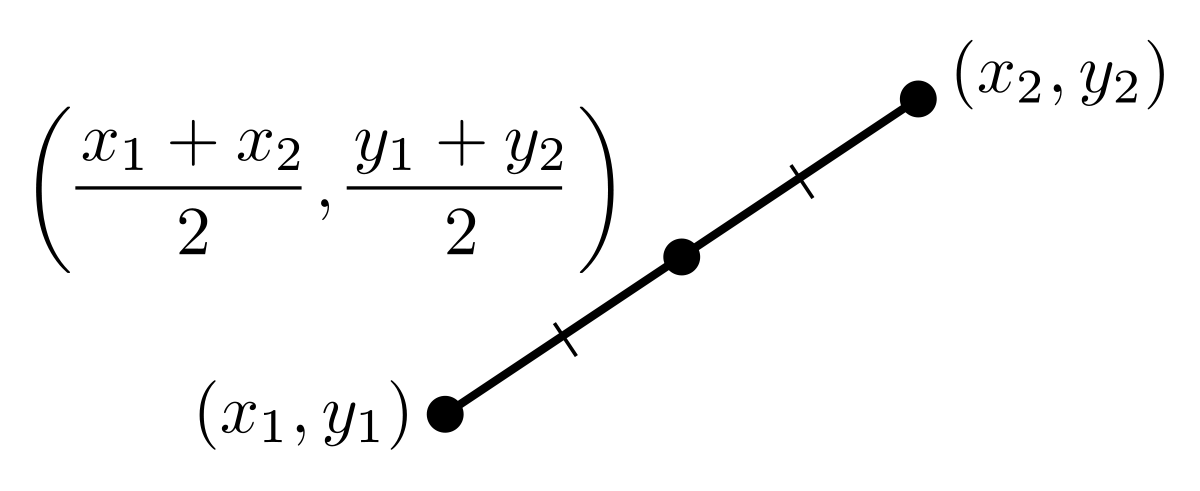
\includegraphics[width=2.60417in,height=\textheight]{img/middle_point.png}
\caption{punto medio}
\end{figure}

\hypertarget{cuxf3mo-calcularla}{%
\subsubsection{Cómo calcularla}\label{cuxf3mo-calcularla}}

Para calcularlo, si tenemos una tabla de frecuencias

\begin{longtable}[]{@{}ll@{}}
\toprule
\(x_i\) & \(n_i\)\tabularnewline
\midrule
\endhead
\(x_1\) & \(n_1\)\tabularnewline
\(x_2\) & \(n_2\)\tabularnewline
\(x_3\) & \(n_3\)\tabularnewline
\(\vdots\) & \(\vdots\)\tabularnewline
\(x_N\) & \(n_N\)\tabularnewline
\bottomrule
\end{longtable}

puesto que cada valor \(x_i\) se repite \(n_i\) veces, calcularemos la
media de la siguiente manera

\[\overline x = \frac{x_1 \cdot n_1 + x_2  \cdot n_2 + x_3  \cdot n_3 +\ldots  + x_N  \cdot n_N}{N} = \frac{1}{N}\sum^{N}_{i=1} x_i  \cdot n_i\]

en el caso de que tengamos una tabla de frecuencias agrupadas por
intervalos

\begin{longtable}[]{@{}lll@{}}
\toprule
\(I_i\) & \(x_i = \frac{x_i + x_{i+1}}{2}\) & \(n_i\)\tabularnewline
\midrule
\endhead
\([l_1, l_2)\) & \(x_1\) & \(n_1\)\tabularnewline
\([l_2, l_3)\) & \(x_2\) & \(n_2\)\tabularnewline
\([l_3, l_4)\) & \(x_3\) & \(n_3\)\tabularnewline
\(\vdots\) & \(\vdots\) & \(\vdots\)\tabularnewline
\([l_{K}, l_{K+1})\) & \(x_K\) & \(n_K\)\tabularnewline
\bottomrule
\end{longtable}

haremos lo mismo pero usando la marca de clase
\(x_i = \frac{l_i + l_{i+1}}{2}\)

\hypertarget{ejemplos}{%
\subsubsection{Ejemplos}\label{ejemplos}}

La siguiente tabla recoge las ventas de 100 sucursales de una empresa

\begin{longtable}[]{@{}llll@{}}
\toprule
ventas (miles) & \(x_i\) & \(n_i\) & \(x_i \cdot n_i\)\tabularnewline
\midrule
\endhead
{[}700, 800) & 750 & 4 & 3000\tabularnewline
{[}800, 900) & 850 & 7 & 5950\tabularnewline
{[}900, 1000) & 950 & 8 & 7600\tabularnewline
{[}1000, 1100) & 1050 & 10 & 10500\tabularnewline
{[}1100, 1200) & 1150 & 12 & 13800\tabularnewline
{[}1200, 1300) & 1250 & 17 & 21250\tabularnewline
{[}1300, 1400) & 1350 & 13 & 17550\tabularnewline
{[}1400, 1500) & 1450 & 10 & 14500\tabularnewline
{[}1500, 1600) & 1550 & 9 & 13950\tabularnewline
{[}1600, 1700) & 1650 & 7 & 11550\tabularnewline
{[}1700, 1800) & 1750 & 2 & 3500\tabularnewline
{[}1800, 1900) & 1850 & 1 & 1850\tabularnewline
\bottomrule
\end{longtable}

calculemos la media

\begin{align*}
\overline x &= \frac{1}{N}\sum^{N}_{i=1} x_i  \cdot n_i\\
&= \frac{750  \cdot  4 + 850  \cdot  7 + 950 \cdot 8 +  \ldots + 1850 \cdot  1}{100}\\
& = \frac{3000  + 5950  + 7600  + 10500 + 13800 + 21250 + 17550 + 14500 + 13950 + 11550 + 3500  + 1850}{100}\\
&=\frac{125000}{100}=1250
\end{align*}

\hypertarget{moda}{%
\subsection{Moda}\label{moda}}

La \textbf{moda} (\(Mo\)) es el valor que aparece con mayor frecuencia
en un conjunto de datos. Si hubiera varios datos con frecuencia máxima
(no hay un único dato con mayor frecuencia sino varios) la moda serían
todos ellos. Por lo tanto la moda puede no ser única.

\hypertarget{cuxf3mo-calcularla-1}{%
\subsubsection{Cómo calcularla}\label{cuxf3mo-calcularla-1}}

Simplemente buscamos el valor o valores con mayor frecuencia absoluta.

\hypertarget{ejemplo-2}{%
\subsubsection{Ejemplo}\label{ejemplo-2}}

La siguente muestra es el resultado realizar una muestra de renta per
capita en un barrio concreto de madrid (en miles de euros anuales
brutos)

\[ 14, 23, 15, 17,12, 0.5, 30, 12, 23, 18, 25, 30, 15, 12, 23 \]

\begin{longtable}[]{@{}ll@{}}
\toprule
renta & \(n_i\)\tabularnewline
\midrule
\endhead
0.5 & 1\tabularnewline
12 & 3\tabularnewline
14 & 1\tabularnewline
17 & 1\tabularnewline
18 & 1\tabularnewline
23 & 3\tabularnewline
30 & 2\tabularnewline
\bottomrule
\end{longtable}

Luego la moda es: \[Mo = 12, 23\]

\hypertarget{mediana}{%
\subsection{Mediana}\label{mediana}}

La mediana \(Me\) representa el valor de la variable de posición central
en un conjunto de datos ordenados.

Si tenemos un número impar de datos, tomamos como mediana simplemente el
valor que ocupe la posición central al ordenarlos, por ejemplo para los
datos

\[1, 2, 3, 4, 5\]

El dato central es \(3\) así que \(Me = 3\).

Si tenemos un número par de datos, al ordenar los datos no encontraremos
un dato central, sino dos, con lo cual tomaremos como mediana la media
entre estos dos datos centrales. Por ejemplo para los datos

\[7, 8, 9, 10, 11, 12 \]

No hay un dato central, podríamos decir que los valores \(9\) y \(10\)
son \emph{centrales} así que tomamos \(Me= (9+10)/2\)

\hypertarget{cuxf3mo-calcularla-2}{%
\subsubsection{Cómo calcularla}\label{cuxf3mo-calcularla-2}}

Si los datos no están en una tabla de frecuencias, haremos lo que hemos
comentado en los párrafos anteriores. Si hemos organizado los datos por
frecuencias, haremos lo siguiente:

Dada una tabla (en la que calculamos tambíen las frecuencias acumuladas)

\begin{longtable}[]{@{}lll@{}}
\toprule
\(x_i\) & \(n_i\) & \(N_i\)\tabularnewline
\midrule
\endhead
\(x_1\) & \(n_1\) & \(N_1\)\tabularnewline
\(x_2\) & \(n_2\) & \(N_2\)\tabularnewline
\(x_3\) & \(n_3\) & \(N_3\)\tabularnewline
\(\vdots\) & \(\vdots\) & \(\vdots\)\tabularnewline
\(x_N\) & \(n_N\) & \(N_N\)\tabularnewline
\bottomrule
\end{longtable}

\begin{enumerate}
\def\labelenumi{\arabic{enumi}.}
\tightlist
\item
  Buscamos el valor que ocupa la \emph{posición central} mirando en la
  tabla cual es el primer dato \(x_i\) cuya frecuencia acumulada supera
  o iguala \(N/2\).
\item
  Si encontramos un dato cuya frecuencia acumulada \(N_i\)
  \textbf{iguala} \(N/2\) tomamos como mediana la media de ese dato
  \(x_i\) y el siguiente \(x_{i+1}\). \(Me = \frac{x_{i} + x_{i+1}}{2}\)
\item
  Si no encontramos uno cuya \(N_i\) iguale a \(N/2\) sino uno que la
  supere directamente, tomamos ese dato como mediana. \(Me = x_i\).
\end{enumerate}

\hypertarget{bibliografuxeda}{%
\section{Bibliografía}\label{bibliografuxeda}}

\begin{itemize}
\tightlist
\item
  John A. Rice. Mathematical Statistics and Data Analysis
\item
  F. M. Dekking, C. Kraailkamp, H. P. Lopuhaa, L. E. Meester. A Modern
  Introduction to Probability and Statistics. Understanding Why and How.
\item
  \url{https://es.wikipedia.org/wiki/Distribuci\%C3\%B3n_Bernoulli}
\item
  \url{https://es.wikipedia.org/wiki/Distribuci\%C3\%B3n_binomial}
\item
  \url{https://es.wikipedia.org/wiki/Distribuci\%C3\%B3n_geom\%C3\%A9trica}
\end{itemize}

\end{document}